\documentclass[10pt]{beamer}
\usepackage[spanish]{babel}
\selectlanguage{spanish} 
\usepackage[utf8]{inputenc}
\usepackage{default}
\usetheme{Montpellier}
%\usecolortheme{dolphin}
\usecolortheme{whale}
\usepackage{graphicx}
\usepackage{float} % supuestamente sirve para las tablas, con [H] se ponen en donde uno quiere
\restylefloat{table} % supuestamente sirve para las tablas, con [H] se ponen en donde uno quiere

\usepackage{subfig}    %para hacer figuras multiples
%\usepackage{hyperref}
\usepackage{cancel}

%\usepackage{wrapfig}
%\newcommand{\director}{Directores:\\Director name}

%\title%[Detecci\'on de Transitorios] % (optional, only for long titles)
%{Series Temporales en Galaxias}
%\subtitle{Detecci\'on de eventos transitorios en im\'agenes}
%\author[S\'anchez]%, Lares, Dom\'{i}nguez] % (optional, for multiple authors)
%{Bruno~S\'anchez\inst{1}\\% \and M.~Lares\inst{2} \and M.~Dom\'{i}nguez\inst{2}\inst{3}}
%\scriptsize{M.~Dom\'{i}nguez\inst{2}\inst{3} \and M.~Lares\inst{2}}}
%\institute[Universidad Nacional de C\'ordoba] % (optional)
%{
%  \inst{1}%
%  Observatorio Astron\'omico\\
%  Universidad Nacional de C\'ordoba
%  \and
%  \inst{2}%
%  Instituto de Astronom\'{i}a Te\'orica y Experimental \\
%  Universidad Nacional de C\'ordoba
%  \and
%  \inst{3}
  %Departamento Astrofisica??
%  University of Texas at Brownsville
%}

\begin{document}


\title[Im\'agenes astron\'omicas]
{Detecci\'on de eventos transitorios en im\'agenes astron\'omicas}
%\subtitle{Gravitational arcs detection and real/bogus classification}
\institute{IATE - CONICET - Universidad Nacional de C\'ordoba (UNC)}
\titlegraphic{
\includegraphics[scale=0.8]{./images/vitraux_h90.png}}
\author{\begin{tabular}{r@{ }l} 
Author:      & Bruno S\'anchez \\[1ex]   & Mariano Dom\'{i}nguez\\ & Marcelo Lares\\ & Mario D\'{i}az \\ & Mart\'{i}n Beroiz%Tania Tagliaferro  \\ & Carlos Valotto
\end{tabular}}
%\date{Date of Presentation}

%\begin{frame}
%  \titlepage
%\end{frame}
\frame{\titlepage}
\begin{frame}
\frametitle{Contents}
\tableofcontents%[sectionstyle=show/hide, 
    %sectionstyle=show/shaded]
\end{frame}
%%%%%%%%%%%%%%%%%%%%%%%%%%%%%%%%%%%%%%%%%%%%%%%%%%%%%%%%%%%%%%%
%%%%%%%%%%%%%%%%%%%%%%%%%%%%%%%%%%%%%%%%%%%%%%%%%%%%%%%%%%%%%%%
\section{Breve introducci\'on}
\frame{
\tableofcontents[ 
    currentsection, 
    %hideothersections, 
    sectionstyle=show/hide, 
    sectionstyle=show/shaded, 
    ]}
%%%%%%%%%%%%%%%%%%%%%%%%%%%%%%%%%%%%%%%%%%%%%%%%%%%%%%%%%%%%%%%
\subsection{Variabilidad Astron\'omica}
%%%%%%%%%%%%%%%%%%%%%%%%%%%%%%%%%%%%%%%%%%%%%%%%%%%%%%%%%%%%%%%
\begin{frame}
La variabilidad en astronom\'{i}a es referida al estudio del cambio del brillo de un 
objeto astron\'omico en el tiempo \pause (\textit{serie temporal}-\textit{curvas de luz}) \\ 
\bigskip
Las series temporales en astronom\'{i}a sirven mayormente para:
\begin{itemize}
\item Clasificaci\'on de objetos 
\item Estudio de NEO's 
\item Estudio de sistemas estelares 
\item Determinaci\'on de distancias 
%\item Comprensi\'on de AGN's 
\item Estudiar expansi\'on del universo
\end{itemize}
\end{frame}
%%%%%%%%%%%%%%%%%%%%%%%%%%%%%%%%%%%%%%%%%%%%%%%%%%%%%%%%%%%%%%%
\begin{frame}
Hay varios tipos de variabilidad:
\begin{itemize}[<+->]
 \item Variabilidad Peri\'odica
 \only<1-1> {\begin{figure}[h] %%curva RRlyr
  %\includegraphics[width=2in,angle=-90]{./../../../tesis/manus/pics/curva_RRLyr.ps}
  \begin{center}
 \includegraphics[bb=0 0 806 559, width=0.7\textwidth]{./images/curva_RRLyr.png}
 % curva_RRLyr.png: 1119x776 pixel, 100dpi, 28.42x19.71 cm, bb=0 0 806 559
\end{center}

 % curva_RRLyr.ps: 595x841 pixel, 72dpi, 20.99x29.67 cm, bb=0 0 595 841
 \caption{\scriptsize{Curva de Luz de una estrella Variable Pulsante Clase RR Lyra. Realizado con datos de CRTSS.}}
 %\label{fig:RRLyr}
\end{figure}}
 \item Variabilidad Transitoria
 \only<2-2>{\begin{figure}[h]  %%curva ptf11kly
  %\includegraphics[width=3in]{./pics/ptf11kly.ps}
  \begin{center}
 \includegraphics[bb=0 0 1043 646, width=0.7\textwidth]{./images/ptf11kly.png}
 % ptf11kly.png: 1043x646 pixel, 72dpi, 36.79x22.79 cm, bb=0 0 1043 646
\end{center}
 % ptf11kly.ps: 1044x647 pixel, 72dpi, 36.83x22.82 cm, bb=0 0 1044 647
 \caption{\scriptsize{Curva de luz de Supernova Tipo Ia, correspondiente al evento PTF11kly. Datos de PTF.}}
%\label{fig:ptfkly_2}
\end{figure}
}
\only<3-3>{\begin{figure}
 \centering
 \includegraphics[width=0.7\textwidth,bb=0 0 93 49]{./images/ptf11kly.jpg}
 % ptf11kly.jpg: 1550x819 pixel, 1200dpi, 3.28x1.73 cm, bb=0 0 93 49
 \caption{\scriptsize{Curva de luz de Supernova Tipo Ia, correspondiente al evento PTF11kly. Datos de PTF.}}
\end{figure}
}
\end{itemize}
\end{frame}
%%%%%%%%%%%%%%%%%%%%%%%%%%%%%%%%%%%%%%%%%%%%%%%%%%%%%%%%%%%%%%%
\subsection{Las Ondas Gravitacionales}
%%%%%%%%%%%%%%%%%%%%%%%%%%%%%%%%%%%%%%%%%%%%%%%%%%%%%%%%%%%%%%%
%%%%%%%%%%%%%%%%%%%%%%%%%%%%%%%%%%%%%%%%%%%%%%%%%%%%%%%%%%%%%%%
\begin{frame}
La teor\'{i}a de la Relatividad General (RG) admite en sus ecuaciones la existencia de \textbf{radiaci\'on gravitatoria}.\\ 
\bigskip
Estas son llamadas \textbf{Ondas Gravitacionales} (GW por sus siglas en ingl\'es).\\ 
Las GW son \textbf{ondas transversales}: las perturbaciones que inducen son en el plano perpendicular a la
direcci\'on de propagaci\'on.\\ \pause
\begin{figure}
 \centering
\begin{center}
 \includegraphics[bb=0 0 391 297, width=0.7\textwidth]{./images/Ondaviajandosobrecuerda2.jpg}
 % Ondaviajandosobrecuerda2.jpg: 391x297 pixel, 72dpi, 13.79x10.48 cm, bb=0 0 391 297
\end{center}

 % Ondaviajandosobrecuerda2.jpg: 391x297 pixel, 72dpi, 13.79x10.48 cm, bb=0 0 391 297
\end{figure}
\end{frame}
%%%%%%%%%%%%%%%%%%%%%%%%%%%%%%%%%%%%%%%%%%%%%%%%%%%%%%%%%%%%%%%
\begin{frame}
La detecci\'on se realiza mediante interfer\'ometros de Michelson\\ \pause 
Para incrementar la precisi\'on de estos aparatos es necesario alargar la longitud de los brazos del interfer\'ometro, y esto ha 
originado la construcci\'on de enormes laboratorios con interfer\'ometros con brazos de kil\'ometros de largo
\begin{figure}[H]  %michelson
   \centering
    \includegraphics[bb=0 0 342 263, width=0.45\textwidth]{./images/10-1.png}
     % 10-1.png: 342x263 pixel, 72dpi, 12.06x9.28 cm, bb=0 0 342 263
 \includegraphics[bb=0 0 642 343, width=0.45\textwidth]{./images/Hanford1.jpg}
 % Hanford1.jpg: 803x429 pixel, 90dpi, 22.66x12.11 cm, bb=0 0 642 343
     %\includegraphics[width=.45\textwidth,bb=14 14 657 358]{./pics/Hanford1.eps}
    %\caption{Interfer\'ometro de LIGO en Hanford}
   %\caption{\scriptsize{Esquema de un interfer\'ometro de Michelson.}}
  %\label{fig:Michelson}
  \end{figure}\pause
 Otros detectores: Virgo, GEO 600, LCGT, AIGO, y LIGO.
\end{frame}
%%%%%%%%%%%%%%%%%%%%%%%%%%%%%%%%%%%%%%%%%%%%%%%%%%%%%%%%%%%%%%%
\begin{frame}
\begin{figure}[h]  %%charliebrown
   %\includegraphics[bb=14 14 241 181, width=0.6\textwidth]{./pics/gw_detector.eps}
   \begin{center}
 \includegraphics[bb=0 0 227 166, width=0.7\textwidth]{./images/gw_detector.png}
 % gw_detector.png: 472x346 pixel, 150dpi, 7.99x5.86 cm, bb=0 0 227 166
  \caption{\scriptsize{Esquema de las perturbaciones inducidas por las GW. Extra\'{i}do de \url{http://www.einstein-online.info/spotlights/gravWav}.}}
\end{center}
 %\label{fig:charliebrown}
 \end{figure}
\end{frame}
%%%%%%%%%%%%%%%%%%%%%%%%%%%%%%%%%%%%%%%%%%%%%%%%%%%%%%%%%%%%%%%
\begin{frame}
Los problemas de localizaci\'on de los eventos utilizando tan s\'olo detectores de GW son importantes.
\begin{figure}[h]
 \centering
 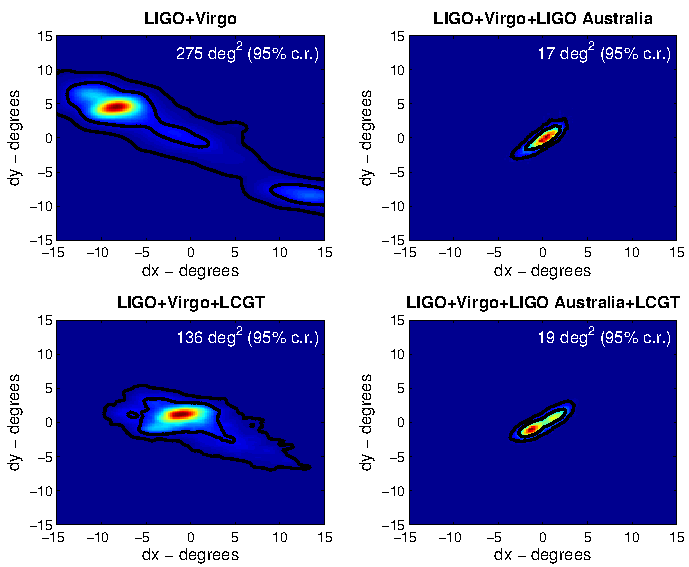
\includegraphics[width=0.7\textwidth]{./images/fig2.png}
 % fig2.eps: 0x0 pixel, 300dpi, 0.00x0.00 cm, bb=   52   197   548   605
 \caption{\scriptsize{Localizaci\'on en el cielo de eventos con S/N baja.}} 
 %Las lineas negras solidas indican una regi\'on con una confidencia del 68\% y 95\%, y 
 %sobre cada figura se muestra que red particular se utiliz\'o.}
 %\label{fig:skyerror1}
\end{figure}
\end{frame}
%%%%%%%%%%%%%%%%%%%%%%%%%%%%%%%%%%%%%%%%%%%%%%%%%%%%%%%%%%%%%%%
\begin{frame}
La detecci\'on de estos eventos entonces necesita \textbf{confirmaci\'on} mediante un m\'etodo independiente.\\
\bigskip
Existe un candidato firme: la colisi\'on y fusi\'on de objetos compactos, como estrellas de neutrones, o 
agujeros negros, denominado \textbf{Kilonova}.\\

\begin{figure}[h]
 \centering
 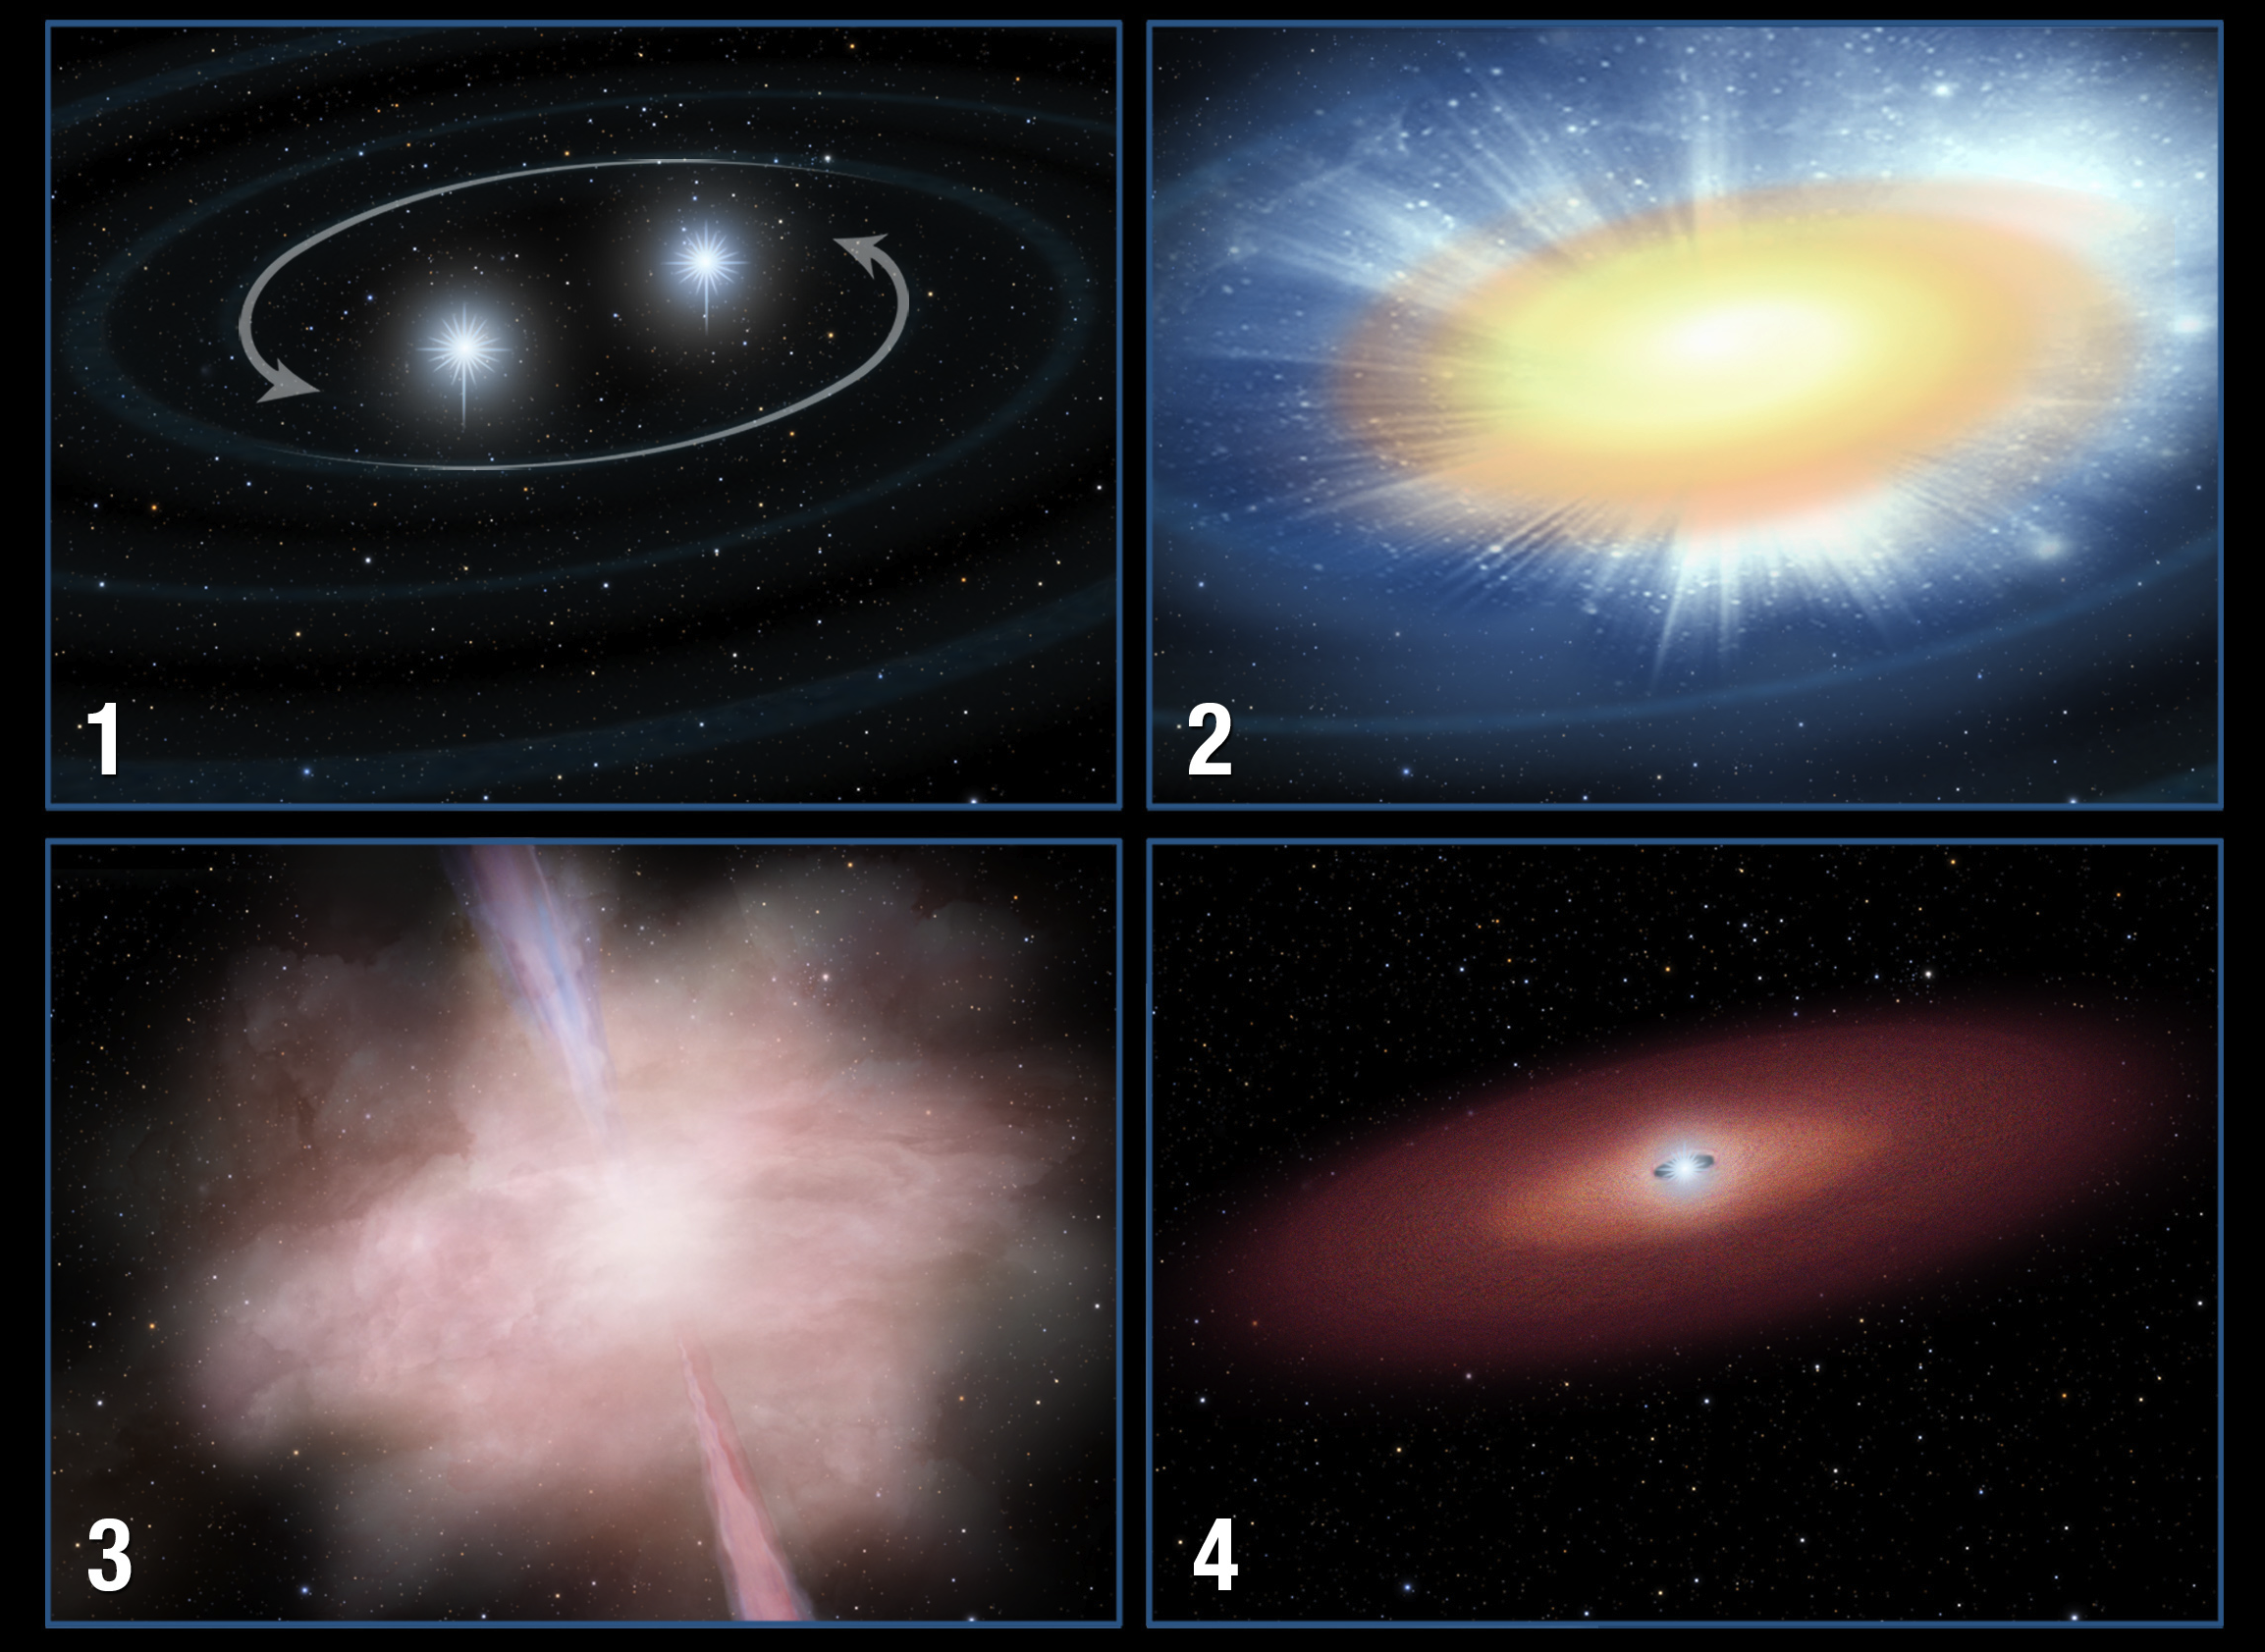
\includegraphics[width=0.5\textwidth,bb=0 0 2307 1683]{./images/merger_model.png}
 % merger_model.ps: 2307x1683 pixel, 72dpi, 81.39x59.37 cm, bb=0 0 2307 1683
 \caption{\scriptsize{Modelo de fusi\'on de objetos compactos: (1) Sistema binario de estrellas de neutrones; 
 (2) concluida la etapa de acercamiento en espiral los objetos toman contacto; 
 (3) los objetos se fusionan disparando un jet en la direcci\'on perpendicular al plano orbital y expulsando material que emite radiaci\'on casi isotr\'opicamente; 
 (4) el material eyectado decae radioactivamente y se apaga formando un disco. Extra\'{i}do de \url{http://www.einstein-online.info/spotlights/gravWav}.}}
 %\label{fig:merger}
\end{figure}
\end{frame}
%%%%%%%%%%%%%%%%%%%%%%%%%%%%%%%%%%%%%%%%%%%%%%%%%%%%%%%%%%%%%%%
\begin{frame}
El evento de fusi\'on posee las siguientes contrapartes electromagn\'eticas:
    \begin{figure}[H]
  \centering
 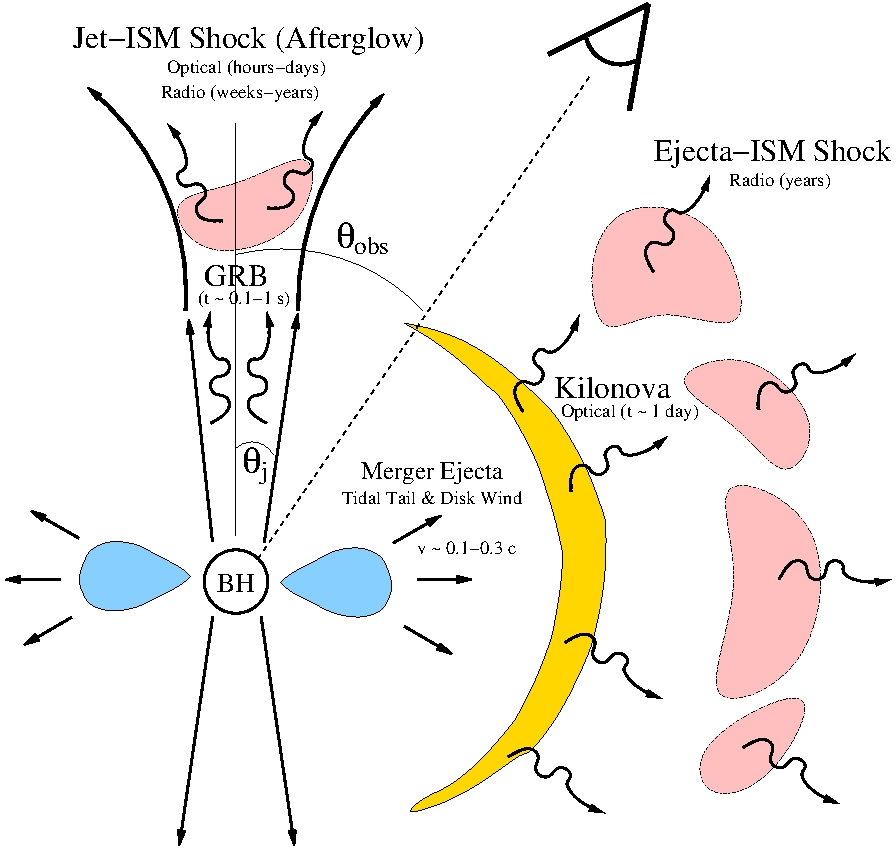
\includegraphics[bb=0 0 645 613, width=0.7\textwidth]{./images/cartoon.jpg}
 \caption{\scriptsize{Esquema de Kilonova, de Metzger \& Berger 2011.}}
 %\label{fig:kilonova}
\end{figure}%}
\end{frame}
%%%%%%%%%%%%%%%%%%%%%%%%%%%%%%%%%%%%%%%%%%%%%%%%%%%%%%%%%%%%%%%
\begin{frame}
Curva de luz del modelo de kilonova
\begin{figure}[!h]
 \centering
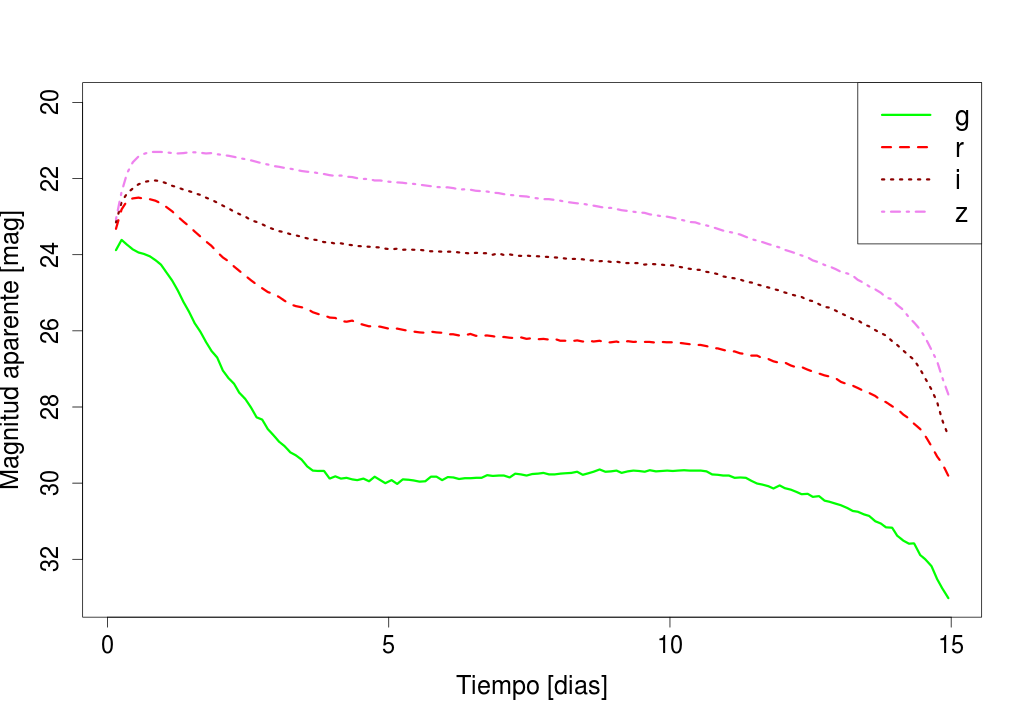
\includegraphics[bb=0 0 1024 720, width=0.7\textwidth]{./images/curva_kilo_abs.png}
 \caption{\scriptsize{Curva de luz de Kilonova. Datos de Barnes \& Kasen 2014 (de la colaboraci\'on de TOROS).}}
 %\label{fig:kilo_lc}
\end{figure}
\end{frame}
%%%%%%%%%%%%%%%%%%%%%%%%%%%%%%%%%%%%%%%%%%%%%%%%%%%%%%%%%%%%%%%
\section{Planteo observacional}
\frame{
\tableofcontents[ 
    currentsection, 
    %hideothersections, 
    sectionstyle=show/hide, 
    sectionstyle=show/shaded, 
    ]}
%%%%%%%%%%%%%%%%%%%%%%%%%%%%%%%%%%%%%%%%%%%%%%%%%%%%%%%%%%%%%%%
\subsection{Simulamos objetos}
%%%%%%%%%%%%%%%%%%%%%%%%%%%%%%%%%%%%%%%%%%%%%%%%%%%%%%%%%%%%%%%
%%%%%%%%%%%%%%%%%%%%%%%%%%%%%%%%%%%%%%%%%%%%%%%%%%%%%%%%%%%%%%%
\begin{frame}
 Resulta que Kilonovas observadas hay UNA.\\ 
 Y es s\'olo un candidato. \\
 Que hace falta para observar una Kilonova??
 \begin{itemize}[<+->]
  \item Telescopio
  \item Muchas observaciones
  \item Detectar variabilidad de corta duraci\'on
  \item Velocidad de procesado de datos
 \end{itemize}
 \pause
 Proyecto TOROS - TORITOS
\begin{figure}
 \centering
 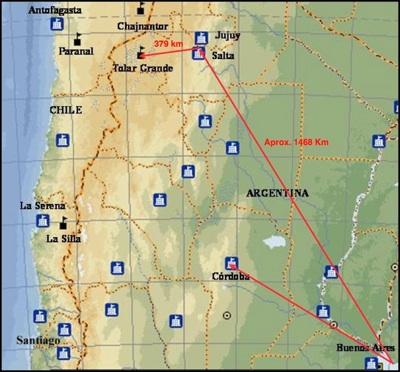
\includegraphics[bb=0 0 400 372, width=0.3\textwidth]{./images/Site.jpg}
 % Site.jpg: 400x372 pixel, 72dpi, 14.11x13.12 cm, bb=0 0 400 372
 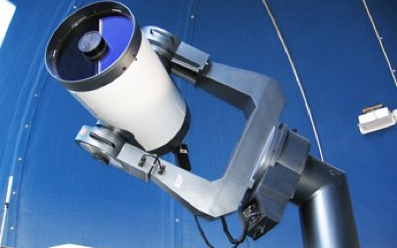
\includegraphics[bb=0 0 159 99, width=0.45\textwidth]{./images/toritos_1.png}
 % toritos_1.png: 397x248 pixel, 180dpi, 5.60x3.50 cm, bb=0 0 159 99
\end{figure}
\end{frame}
%%%%%%%%%%%%%%%%%%%%%%%%%%%%%%%%%%%%%%%%%%%%%%%%%%%%%%%%%%%%%%%
\begin{frame}
 \begin{itemize}
  \item TORITOS comenzar\'{i}a a trabajar para el mes de septiembre, 
 donde aLIGO va a tener una corrida cient\'{i}fica de un mes aproximadamente.
 \item Para trabajar con un telescopio en el cerro necesitamos software que minimize la interacci\'on
 con un ser humano.
 \item  Junto con Mart\'{i}n Beroiz trabajamos en el desarrollo del \textit{pipeline} de 
 trabajo del instrumento.
 \item A\'un as\'{i} necesitamos saber de antemano sobre el \textit{data product} \pause
 \item La respuesta a esto son simulaciones de datos con cadencia temporal.
 \end{itemize}
\end{frame}
%%%%%%%%%%%%%%%%%%%%%%%%%%%%%%%%%%%%%%%%%%%%%%%%%%%%%%%%%%%%%%%
\begin{frame}
Para simular im\'agenes tuvimos que tener en cuenta detalles t\'ecnicos como:
\begin{itemize}%[<+->]
 \item Difracci\'on
 \item PSF
 \item Fondo del cielo
 \item Pixelizado
 \item Escalas fotom\'etricas
% \item Tiempos de c\'omputo
\end{itemize}
\end{frame}
%%%%%%%%%%%%%%%%%%%%%%%%%%%%%%%%%%%%%%%%%%%%%%%%%%%%%%%%%%%%%%%
\begin{frame}
¿Cu\'al es la falsa?
\begin{center}
 \includegraphics[width=0.48\textwidth]{./images/campo1.jpg}
 \includegraphics[width=0.48\textwidth]{./images/campo2.jpg}
 % campo1.jpg: 495x444 pixel, 72dpi, 17.46x15.66 cm, bb=0 0 495 444
\end{center}
\end{frame}
%%%%%%%%%%%%%%%%%%%%%%%%%%%%%%%%%%%%%%%%%%%%%%%%%%%%%%%%%%%%%%%
\begin{frame}
Diferentes galaxias
\begin{figure}
 \centering
 \includegraphics[width=\textwidth,bb=0 0 856 473]{./images/ds9.jpg}
 % ds9.ps: 856x473 pixel, 72dpi, 30.20x16.69 cm, bb=0 0 856 473
% \caption{Im\'agenes astron\'omicas simuladas con nuestro software. En el centro de cada una se encuentra una galaxia. La de la izquierda 
% corresponde a una galaxia tipo el\'{i}ptica, la de la derecha en cambio corresponde a una galaxia tipo disco.}
\end{figure}
\end{frame}
%%%%%%%%%%%%%%%%%%%%%%%%%%%%%%%%%%%%%%%%%%%%%%%%%%%%%%%%%%%%%%%
\subsection{An\'alisis de las im\'agenes simuladas}
%%%%%%%%%%%%%%%%%%%%%%%%%%%%%%%%%%%%%%%%%%%%%%%%%%%%%%%%%%%%%%%
\begin{frame}\frametitle{An\'alisis de las im\'agenes}
Para el an\'alisis de las im\'agenes empleamos:
\begin{itemize}
 \item Fotometr\'{i}a de Apertura \pause
 \begin{itemize}
  \item Consta de utilizar ``aperturas'' para encerrar las fuentes astron\'omicas y calcular
  la energ\'{i}a recibida %\pause
  \item $m_1 - m_2 = -2.5 log_{10}\left(\frac{E_1}{E_2}\right)$ %\pause
\begin{figure}
  \begin{center}
 \includegraphics[width=0.4\textwidth]{./images/apertures.png}
 % apertures.png: 680x472 pixel, 72dpi, 23.99x16.65 cm, bb=0 0 680 472
\end{center}
\end{figure}
 \end{itemize}
 \item Fotometr\'{i}a de Diferencias \pause
 \begin{itemize}
  \item Consta de ``restar'' dos im\'agenes astron\'omicas%\pause
  \item Formalmente involucra an\'alisis de Fourier para calibrar ambas im\'agenes%\pause
  \item Utilizamos resta directa ya que nuestras im\'agenes de por s\'{i} estaban calibradas%\pause
 \end{itemize}
\end{itemize}
\end{frame}
%%%%%%%%%%%%%%%%%%%%%%%%%%%%%%%%%%%%%%%%%%%%%%%%%%%%%%%%%%%%%%%
\begin{frame}\frametitle{Algunos n\'umeros}
Resumiendo en n\'umeros nuestras simulaciones:
\begin{itemize}%[<+->]
% \item Exploramos 288 puntos del espacio de par\'ametros
\item 3555 series temporales obtenidas
\item 182490 im\'agenes simuladas
\item M\'as de 28500 curvas de luz
\item Se crearon otras 182490 im\'agenes de fotometr\'{i}a de diferencias
\item 5,1 Terabytes de espacio total de memoria utilizado.
\end{itemize}
\end{frame}
%%%%%%%%%%%%%%%%%%%%%%%%%%%%%%%%%%%%%%%%%%%%%%%%%%%%%%%%%%%%%%%
\subsection{La Construcci\'on de una Figura de M\'erito}
%%%%%%%%%%%%%%%%%%%%%%%%%%%%%%%%%%%%%%%%%%%%%%%%%%%%%%%%%%%%%%%
\begin{frame}\frametitle{La Construcci\'on de una Figura de M\'erito}
 Se le llama Figura de M\'erito a un estimador (o a un conjunto de estimadores) que caracterizan
el rendimiento de un test estad\'{i}stico.
En el trabajo lidiamos con m\'etodos que realizan m\'ultiples pruebas por hip\'otesis
Todo proceso de este tipo tiene dos posibles errores: 
%{%
%\newcommand{\mc}[3]{\multicolumn{#1}{#2}{#3}}
\begin{center}
\begin{tabular}{|c|c|l|}
\hline
- & \multicolumn{2}{c|}{Decisi\'on}\\
\hline \hline
Condici\'on Real & Rechazar $H_0$ & \multicolumn{1}{c|}{Mantener $H_0$}\\
\hline
$H_0$ Verdadera & Error de Tipo I & \multicolumn{1}{c|}{Acierto}\\
\hline
$H_0$ Falsa & Acierto & \multicolumn{1}{c|}{Error de Tipo II}\\
\hline
\end{tabular}
\end{center}
%}%
\end{frame}
%%%%%%%%%%%%%%%%%%%%%%%%%%%%%%%%%%%%%%%%%%%%%%%%%%%%%%%%%%%%%%%
\begin{frame} \frametitle{La Construcci\'on de una Figura de M\'erito}
 Los estad\'{i}sticos que miden el rendimiento de un test de decisi\'on son FDR, TPR, y FPR.
\begin{itemize}
 \item FDR (o \textit{Tasa de Falsos Descubrimientos}) corresponde a la probabilidad 
 de cometer un error de Tipo I habiendo obtenido como resultado el rechazo de $H_0$
 \item TPR (o \textit{Tasa de Positivos Verdaderos}) corresponde a la probabilidad de 
 rechazar la $H_0$ dado que es falsa, o bien uno menos la probabilidad de cometer un Error de Tipo I
\item FPR (o \textit{Tasa de Falsos Positivos}) el cual es la probabilidad de cometer un error de Tipo II
\end{itemize}
\end{frame}
%%%%%%%%%%%%%%%%%%%%%%%%%%%%%%%%%%%%%%%%%%%%%%%%%%%%%%%%%%%%%%%
\begin{frame} \frametitle{La Construcci\'on de una Figura de M\'erito}
 \begin{columns}[T]
\begin{column}{0.48\textwidth}
 Las tasas de FPR y TPR dependen del valor umbral que se aplique a un dado m\'etodo.\\ 
 El valor umbral es qui\'en procede a decidir si hubo o no detecci\'on y se asocia principalmente
 con el valor de confidencia que se pida a un test.\\ 
 Las tasas de FPR y TPR poseen un balance que se caracteriza por la \textit{Respuesta Caracter\'{i}stica del Operador}.\\ 
 Y el estimador de rendimiento que usaremos ser\'a el AUC (\textit{\'Area Bajo la Curva})
 \end{column}
 \begin{column}{0.55\textwidth}
 \begin{figure}
 \centering
 \includegraphics[width=\textwidth]{./images/ROC.png}
 % ROC.ps: 504x504 pixel, 72dpi, 17.78x17.78 cm, bb=0 0 504 504
 \caption{\scriptsize{Curva ROC}}
 %\label{fig:roc}
\end{figure}\pause
\end{column}
 \end{columns}
\end{frame}
%%%%%%%%%%%%%%%%%%%%%%%%%%%%%%%%%%%%%%%%%%%%%%%%%%%%%%%%%%%%%%%
\section{Primeros resultados}
%%%%%%%%%%%%%%%%%%%%%%%%%%%%%%%%%%%%%%%%%%%%%%%%%%%%%%%%%%%%%%%
\frame{
\tableofcontents[ 
    currentsection, 
    %hideothersections, 
    sectionstyle=show/hide, 
    sectionstyle=show/shaded, 
    ]}
%%%%%%%%%%%%%%%%%%%%%%%%%%%%%%%%%%%%%%%%%%%%%%%%%%%%%%%%%%%%%%%
\subsection{Figura de M\'erito para los tests (Fotometr\'{i}a de apertura)}
%%%%%%%%%%%%%%%%%%%%%%%%%%%%%%%%%%%%%%%%%%%%%%%%%%%%%%%%%%%%%%%
\begin{frame}\frametitle{Figura de M\'erito para los Tests}
 \begin{figure}
 \centering
 \includegraphics[width=0.7\textwidth]{./images/fig_02.pdf}
 % FOM.ps: 504x504 pixel, 72dpi, 17.78x17.78 cm, bb=0 0 504 504
 \caption{\scriptsize{Curva ROC de nuestros tests de variabilidad.}}
 %\label{fig:fom}
\end{figure}
\end{frame}
%%%%%%%%%%%%%%%%%%%%%%%%%%%%%%%%%%%%%%%%%%%%%%%%%%%%%%%%%%%%%%%
\begin{frame}\frametitle{Figura de M\'erito para los Tests}
 \begin{figure}
 \centering
 \includegraphics[width=0.3\textwidth]{./images/fig_02.pdf}
 % FOM.ps: 504x504 pixel, 72dpi, 17.78x17.78 cm, bb=0 0 504 504
 \caption{\scriptsize{Curva ROC de nuestros tests de variabilidad.}}
 %\label{fig:fom}
\end{figure}
\begin{center}
\begin{tabular}{|c|c|c|c|c|c|c|}
\hline
Test & T1C & T2C & T3C & VC & VD & D\\
\hline %\hline
AUC & 0.55 & 0.50 & 0.55 & 0.61 & 0.61 & 0.49\\
\hline
\end{tabular}
%\label{tab:fom}
\end{center}
\end{frame}
%%%%%%%%%%%%%%%%%%%%%%%%%%%%%%%%%%%%%%%%%%%%%%%%%%%%%%%%%%%%%%%
%%%%%%%%%%%%%%%%%%%%%%%%%%%%%%%%%%%%%%%%%%%%%%%%%%%%%%%%%%%%%%%
\subsection{Fotometr\'{i}a de Diferencias}
%%%%%%%%%%%%%%%%%%%%%%%%%%%%%%%%%%%%%%%%%%%%%%%%%%%%%%%%%%%%%%%
\begin{frame} \frametitle{Resultados de la Fotometr\'{i}a de Diferencias}
 El nivel de corte fue de 2$\sigma$
 Hallamos:
  \begin{itemize}%[<+->]
    \item Para la Muestra de Control (sin kilonova)
      \begin{itemize}
	\item 1231 detecciones sobre un total de 1440 series temporales
	\item 85\% de falsas detecciones
      \end{itemize}
    \item Para la Muestra con Kilonova
      \begin{itemize}
	\item 1862 detecciones en un total de 2115 series temporales
	\item 90\% de detecciones certeras
	\item 68\% de objetos esp\'ureos.
      \end{itemize}
  \end{itemize}
 Se puede ver que le erramos por bastante.\\
 El problema es que el nivel de corte es muy bajo, pero un corte m\'as 
 alto nos har\'{i}a perder las Kilonovas que nos est\'an llamando por ah\'{i} \\ \pause
 Que hacer??
\end{frame}
%%%%%%%%%%%%%%%%%%%%%%%%%%%%%%%%%%%%%%%%%%%%%%%%%%%%%%%%%%%%%%%
%%%%%%%%%%%%%%%%%%%%%%%%%%%%%%%%%%%%%%%%%%%%%%%%%%%%%%%%%%%%%%%
\section{Real/Bogus: Una soluci\'on con Machine Learning}
%%%%%%%%%%%%%%%%%%%%%%%%%%%%%%%%%%%%%%%%%%%%%%%%%%%%%%%%%%%%%%%
\frame{
\tableofcontents[ 
    currentsection, 
    %hideothersections, 
    sectionstyle=show/hide, 
    sectionstyle=show/shaded, 
    ]}
%%%%%%%%%%%%%%%%%%%%%%%%%%%%%%%%%%%%%%%%%%%%%%%%%%%%%%%%%%%%%%%
\subsection{Que es Machine Learning?} %the concept of a learning algorithm.
%%%%%%%%%%%%%%%%%%%%%%%%%%%%%%%%%%%%%%%%%%%%%%%%%%%%%%%%%%%%%%%
\begin{frame} \frametitle{Statistical Learning}
Hoy en d\'{i}a mucha ciencia se hace a trav\'es de lo que \textit{los datos dicen}:\\
Extraer ese contenido de informaci\'on es lo que significa \textbf{aprender de los datos} con Machine Learning (ML):\\
%\pause
%\begin{itemize}[<+->]
% \item 
%\vspace{1cm}
\centering
\textbf{Supervised learning}
% \only<1-2>{
 \begin{figure}
 \includegraphics[bb=0 0 3506 2549,scale=0.065]{./images/supervised.png}
 % supervised.png: 3506x2549 pixel, 72dpi, 123.67x89.91 cm, bb=0 0 3506 2549
\end{figure}
\end{frame}
%%%%%%%%%%%%%%%%%%%%%%%%%%%%%%%%%%%%%%%%%%%%%%%%%%%%%%%%%%%%%%%
\subsection{Algoritmos implementados} %the concept of a learning algorithm.
%%%%%%%%%%%%%%%%%%%%%%%%%%%%%%%%%%%%%%%%%%%%%%%%%%%%%%%%%%%%%%%
%%%%%%%%%%%%%%%%%%%%%%%%%%%%%%%%%%%%%%%%%%%%%%%%%%%%%%%%%%%%%%%%
\begin{frame} \frametitle{Algoritmos implementados}
Lo que queremos entonces es aprender a diferenciar un transitorio real de uno falso.\\ 
%\pause
Estos problemas se atacan utilizando las llamadas \textit{\textbf{features}} (en la jerga de ML)
los cuales son los observables asociados a un set de datos
-llamado \textit{\textbf{set de entrenamiento}}- desde el cual el algoritmo debe construir un \textit{\textbf{modelo}}.\\ %\pause
Nosotros usamos tres algoritmos cl\'asicos del ML:
\begin{itemize}%[<+->]
 \item \textbf{Naive Bayes}
 \only<3>{
 Usa el teorema de Bayes para estimar probabilidads de pertenecer a cada clase:
 \\ 
 %\begin{displaymath}
 % P(A|B)P(B) = P(B|A)P(A)
 %\end{displaymath}
%This is a symetrical relationship between two random variables, and
%its ocurrence probabilities.
%Using this it can be estimated a probability of belonging to 
%a given class for a new observation, 
%using the information given in the previous experience:
\begin{displaymath}
 P(c=c_i|\vec{f}) = \frac{P(\vec{f}|c=c_i)P(c=c_i)}{P(\vec{f})}
\end{displaymath}
}
 \item  \textbf{Logistic Regression}
 \only<4>{Este algoritmo asume que las probabilidades de pertenecer a una dada clase
 puede ser linealmente interpolada luego de una transformaci\'on muy simple:
 \begin{displaymath}
  logi(p_i) = \ln(\frac{p_i}{1-p_i}) = \alpha + \beta \times \vec{f}_i
 \end{displaymath}
%where $logi$ is the \textit{logistic function}, $p_i$ the probability of
%belonging to a given class, and again $\vec{f}$ is the features of each data point.
}
\item \textbf{Random Forest}
\only<5>{
Este algoritmo usa muchos \'arboles de decisi\'on, y
posee dos par\'ametros importantes: $N_{tree}$ el n\'umero de 
\'arboles de decisi\'on, y $N_f$ el n\'umero de features al 
azar en cada \'arbol.\\ 
Despu\'es del entrenamiento la clasificaci\'on es calculada en una
votaci\'on entre todos los \'arboles.}
\end{itemize}
\end{frame}
%%%%%%%%%%%%%%%%%%%%%%%%%%%%%%%%%%%%%%%%%%%%%%%%%%%%%%%%%%%%%%%
%%%%%%%%%%%%%%%%%%%%%%%%%%%%%%%%%%%%%%%%%%%%%%%%%%%%%%%%%%%%%%%
\subsection{Real/Bogus}
%%%%%%%%%%%%%%%%%%%%%%%%%%%%%%%%%%%%%%%%%%%%%%%%%%%%%%%%%%%%%%%
%%%%%%%%%%%%%%%%%%%%%%%%%%%%%%%%%%%%%%%%%%%%%%%%%%%%%%%%%%%%%%%
%%%%%%%lots of things missing here commented
%%%%%%%%%%%%%%%%%%%%%%%%%%%%%%%%%%%%%%%%%%%%%%%%%%%%%%%%%%%%%%%
\begin{frame}\frametitle{Construimos el set de entrenamiento}
Simulamos nuevamente datos, produciendo un conjunto balanceado de 9202 \textit{bogus} y 9120 \textit{reals}.
%\pause
\begin{figure}
 \centering
 \includegraphics[scale=1]{../../../Doctorado/codigos/scipycodes/image-simulation-and-analysis/bogus/obj_002.png}
 \includegraphics[scale=1]{../../../Doctorado/codigos/scipycodes/image-simulation-and-analysis/bogus/obj_011.png}
 \includegraphics[scale=1]{../../../Doctorado/codigos/scipycodes/image-simulation-and-analysis/bogus/obj_013.png}
 \includegraphics[scale=1]{../../../Doctorado/codigos/scipycodes/image-simulation-and-analysis/bogus/obj_018.png}
 % obj_002.png: 64x64 pixel, 72dpi, 2.26x2.26 cm, bb=0 0 64 64
 \caption{Estampillas de objetos \textit{bogus} simulados.}
 \label{fig:bogus}
\end{figure}
\begin{figure}
 \centering
 \includegraphics[scale=1]{../../../Doctorado/codigos/scipycodes/image-simulation-and-analysis/real/robj_0025.png}
 \includegraphics[scale=1]{../../../Doctorado/codigos/scipycodes/image-simulation-and-analysis/real/robj_0041.png}
 \includegraphics[scale=1]{../../../Doctorado/codigos/scipycodes/image-simulation-and-analysis/real/robj_0040.png}
 \includegraphics[scale=1]{../../../Doctorado/codigos/scipycodes/image-simulation-and-analysis/real/robj_0115.png}
 % obj_002.png: 64x64 pixel, 72dpi, 2.26x2.26 cm, bb=0 0 64 64
 \caption{Objetos \textit{reales} simulados.}
 \label{fig:reals}
\end{figure}
\end{frame}
%%%%%%%%%%%%%%%%%%%%%%%%%%%%%%%%%%%%%%%%%%%%%%%%%%%%%%%%%%%%%%%
\begin{frame}\frametitle{Procedimiento}
\begin{itemize}[<+->]
 \item Implementamos un \textbf{vectorizador}, el cual simplemente usa datos de los pixeles
y extrae un enorme conjunto de features -llega hasta 3000 features-, 
y usamos un conjunto reducido de \textbf{1028 features}.
 \item Luego usamos el \textbf{WEKA Explorer suit} y analizamos los features.
El suit tiene muchas herramientas de ML para jugar, incluyendo \textbf{selecci\'on de features}.
 \item Usamos dos rutinas: PCA, y \textit{CfSubsetEval} de Hall (1998). Esto reduce el conjunto de 1028
features principalmente para descartar interdependencias.
 \item PCA arroj\'o 310 \textit{principal components}, y nos proporcion\'o la matriz de transformaci\'on de
 los datos, y los vectores de features ya proyectados al espacio de las PC.
 \item El m\'etodo de \textit{CfSubsetEval} arroj\'o 39 features \'utiles.
\end{itemize}
\end{frame}
%%%%%%%%%%%%%%%%%%%%%%%%%%%%%%%%%%%%%%%%%%%%%%%%%%%%%%%%%%%%%%%
\begin{frame}\frametitle{K-fold cross validation}
 La perfomance de los m\'etodos se calcul\'o usando \textit{K-Fold Cross Validation}, 
 esto es dividir los datos en \textbf{K porciones muestreadas al azar}, entrenar
 en K-1 porciones y testear sobre la porci\'on restante. 
 \begin{figure}
 \includegraphics[width=0.6\textwidth,bb=0 0 300 137,keepaspectratio=true]{./images/k-fold.jpg}
 % k-fold.jpg: 471x215 pixel, 113dpi, 10.59x4.83 cm, bb=0 0 300 137
\end{figure}
 %\pause
 Esto se hace K veces, y esto arroja K medidas de perfomance, 
 que es de donde se calculan los estad\'{i}sticos TPR y FPR.
\end{frame}
%%%%%%%%%%%%%%%%%%%%%%%%%%%%%%%%%%%%%%%%%%%%%%%%%%%%%%%%%%%%%%%
\begin{frame}[c, squeeze] \frametitle{Resultados muestra completa de features}
\begin{columns}
\begin{column}{0.3\textwidth}
\begin{center}
\textbf{Naive Bayes} 
\begin{figure}
 \includegraphics[bb=0 0 512 512,scale=0.16]{./images/RB_fullset_NB.png}
 % RB_fullset_NB.png: 512x512 pixel, 72dpi, 18.06x18.06 cm, bb=0 0 512 512
\end{figure}
\end{center}
\end{column}
\begin{column}{0.3\textwidth}
\begin{center}
\textbf{Random Forest}
\begin{figure}
 \includegraphics[bb=0 0 512 512,scale=0.16]{./images/RB_fullset_RF.png}
 % RB_fullset_RF.png: 512x512 pixel, 72dpi, 18.06x18.06 cm, bb=0 0 512 512
\end{figure}
\end{center}
\end{column}
\begin{column}{0.34\textwidth}
 \begin{figure}
 \includegraphics[bb=0 0 480 480,scale=0.249]{./images/full_sample_RB.png}
 % full_sample_RB.png: 480x480 pixel, 72dpi, 16.93x16.93 cm, bb=0 0 480 480
\end{figure}
\end{column}
\end{columns}
\end{frame}
%%%%%%%%%%%%%%%%%%%%%%%%%%%%%%%%%%%%%%%%%%%%%%%%%%%%%%%%%%%%%%%
\begin{frame}[c, squeeze] \frametitle{Resultados para transformada con PCA}
%\only<1>{
\scriptsize
 \begin{columns}
\begin{column}{0.5\textwidth}
\begin{center}
\textbf{Naive Bayes} 
\begin{figure}
 \includegraphics[bb=0 0 512 512,scale=0.136]{./images/RB_PCAset_NB.png}
 % RB_PCAset_NB.png: 512x512 pixel, 72dpi, 18.06x18.06 cm, bb=0 0 512 512
\end{figure}
\textbf{Logistic Regression} %results for PCA features:\pause
\begin{figure}
 \includegraphics[bb=0 0 512 512,scale=0.136]{./images/RB_PCAset_LR.png}
 % RB_PCAset_LR.png: 512x512 pixel, 72dpi, 18.06x18.06 cm, bb=0 0 512 512
\end{figure}
\end{center}
\end{column}

\begin{column}{0.5\textwidth}
\begin{center}
\textbf{Random Forest}% results for PCA features:\pause
\begin{figure}
 \includegraphics[bb=0 0 512 512,scale=0.136]{./images/RB_PCAset_RF.png}
 % RB_PCAset_RF.png: 512x512 pixel, 72dpi, 18.06x18.06 cm, bb=0 0 512 512
\end{figure}

 \begin{figure}
 \centering
 \includegraphics[bb=0 0 480 480,scale=0.2]{./images/PCA_RB.png}
 % PCA_RB.png: 480x480 pixel, 72dpi, 16.93x16.93 cm, bb=0 0 480 480
\end{figure}
%}
\end{center}
\end{column}
\end{columns}
\end{frame}
%%%%%%%%%%%%%%%%%%%%%%%%%%%%%%%%%%%%%%%%%%%%%%%%%%%%%%%%%%%%%%%
\begin{frame}[c, squeeze] \frametitle{Resultados features seleccionados con Cfs}
 \scriptsize
 \begin{columns}\begin{column}{0.5\textwidth}
\begin{center}
 \textbf{Naive Bayes} 
 \begin{figure}
 \centering
 \includegraphics[bb=0 0 512 512,scale=0.14]{./images/RB_Cfsset_NB.png}
 % RB_Cfsset_NB.png: 512x512 pixel, 72dpi, 18.06x18.06 cm, bb=0 0 512 512
\end{figure}
\textbf{Logistic Regression} %results for best features:\pause
\begin{figure}
 \centering
 \includegraphics[bb=0 0 512 512,scale=0.14]{./images/RB_Cfsset_LR.png}
 % RB_Cfsset_LR.png: 512x512 pixel, 72dpi, 18.06x18.06 cm, bb=0 0 512 512
\end{figure}
\end{center}
\end{column}
\begin{column}{0.5\textwidth}
\begin{center}
\textbf{Random Forest} %results for best features:\pause
\begin{figure}
 \centering
 \includegraphics[bb=0 0 512 512,scale=0.14]{./images/RB_Cfsset_RF.png}
 % RB_Cfsset_RF.png: 512x512 pixel, 72dpi, 18.06x18.06 cm, bb=0 0 512 512
\end{figure}

\begin{figure}
 \centering
 \includegraphics[bb=0 0 480 480,scale=0.2]{./images/Cfs_RB.png}
 % Cfs_RB.png: 480x480 pixel, 72dpi, 16.93x16.93 cm, bb=0 0 480 480
\end{figure}

\end{center} 
\end{column}
\end{columns}
\end{frame}
%%%%%%%%%%%%%%%%%%%%%%%%%%%%%%%%%%%%%%%%%%%%%%%%%%%%%%%%%%%%%%%
%%%%%%%%%%%%%%%%%%%%%%%%%%%%%%%%%%%%%%%%%%%%%%%%%%%%%%%%%%%%%%%
\section{Conclusiones \& el trabajo a futuro}
%%%%%%%%%%%%%%%%%%%%%%%%%%%%%%%%%%%%%%%%%%%%%%%%%%%%%%%%%%%%%%%
\frame{
\tableofcontents[ 
    currentsection, 
    %hideothersections, 
    sectionstyle=show/hide, 
    sectionstyle=show/shaded, 
    ]}
%%%%%%%%%%%%%%%%%%%%%%%%%%%%%%%%%%%%%%%%%%%%%%%%%%%%%%%%%%%%%%%
\begin{frame}%[allowframebreaks]
\frametitle{Resumen y conclusiones}
\begin{itemize}[<+->]
\item Implementamos algoritmos de ML para clasificar im\'agenes, 
usando vectorizadores y m\'etodos de selecci\'on de features.
\item Los resultados son esperanzadores, y pueden ser aplicados de forma simple y con la posibilidad de 
determinar errores con confianza.
\item La flexibilidad que tiene esta soluci\'on (especialmente por el vectorizador) hace
que sea expandible a otras situaciones nuevas.
\end{itemize}
\end{frame}
%%%%%%%%%%%%%%%%%%%%%%%%%%%%%%%%%%%%%%%%%%%%%%%%%%%%%%%%%%%%%%%
\begin{frame}
 \frametitle{Trabajo a futuro}
 \begin{itemize}[<+->]
 \item Correr estos clasificadores contra bases de datos p\'ublicas, tales como PTF (trabajo en preparaci\'on)
 \item Hacer \textit{fine tuning} de los clasificadores
  \item Usarlo para TOROS/TORITOS (deployment on spring).
\end{itemize}
\begin{center}
\pause
\textbf{PREGUNTAS?? :D}
\end{center}
\end{frame}
%%%%%%%%%%%%%%%%%%%%%%%%%%%%%%%%%%%%%%%%%%%%%%%%%%%%%%%%%%%%%%%
%%%%%%%%%%%%%%%%%%%%%%%%%%%%%%%%%%%%%%%%%%%%%%%%%%%%%%%%%%%%%%%

\end{document}



